\chapter{序論}
\label{chap:introduction}

\section{背景}

近年,スマートフォンの急速な普及により数多くのアプリケーションが開発され,人々が毎日利用している,そのアプリケーションの開発には人々が感じている課題の洗い出し,適切な仕様の確定,使いやすいインタフェースの設計,実装など専門的で複雑な工程が多数存在する.中でもインタフェース設計とその実装は開発全体の中で設計段階で45%,実装段階で50%,保守段階で37%の時間を占めると言われている.\cite{myers1992survey}

またデザインカンパニーであるGoodpatchの社長である土屋は創業の原点について次のように述べており,デザインの重要性について述べている.\begin{quotation}
Goodpatchは2011年にUIデザインに特化したデザイン会社としてスタートしました。2011年に起業前に渡ったサンフランシスコでは創業期のInstagramやUber、Airbnbなど多くのスタートアップの共同創業者にデザイナーがおり、ベータ版からUIデザインに力を入れ、ユーザー体験を最初から考え、デザインを重要な差別化要素としてプロダクト開発を行っておりました。日本の環境と大きなギャップを感じた土屋は日本に帰り、創業したことがGoodpatchの原点です。\cite{goodpatchwhydesign}
\end{quotation}


大手企業の大規模開発では社内に専門知識を持ったデザイナが在籍していたり,Goodpatchのようなデザインカンパニーと共に設計を行うことが可能であるが専門のデザイナが在籍しないスタートアップ企業やインディーズ開発,個人開発ではこれらを行うのは非常に困難である.


また日本においてはデザインの認識が装飾などの表層的なものであると誤解されている.\cite{goodpatchwhydesign}本来のデザインの役割である本質的な価値を見出し、価値を最大化させること。つまり、本来のデザインとは、具象と抽象を行き来し戦略、要件、構造、骨格、表層全ての設計をすることであるとGarretのUX五段階モデル(図\ref{fig:garretuxmodel})で述べられている.

\begin{figure}[htbp]
  \begin{minipage}{\hsize}
    \begin{center}
       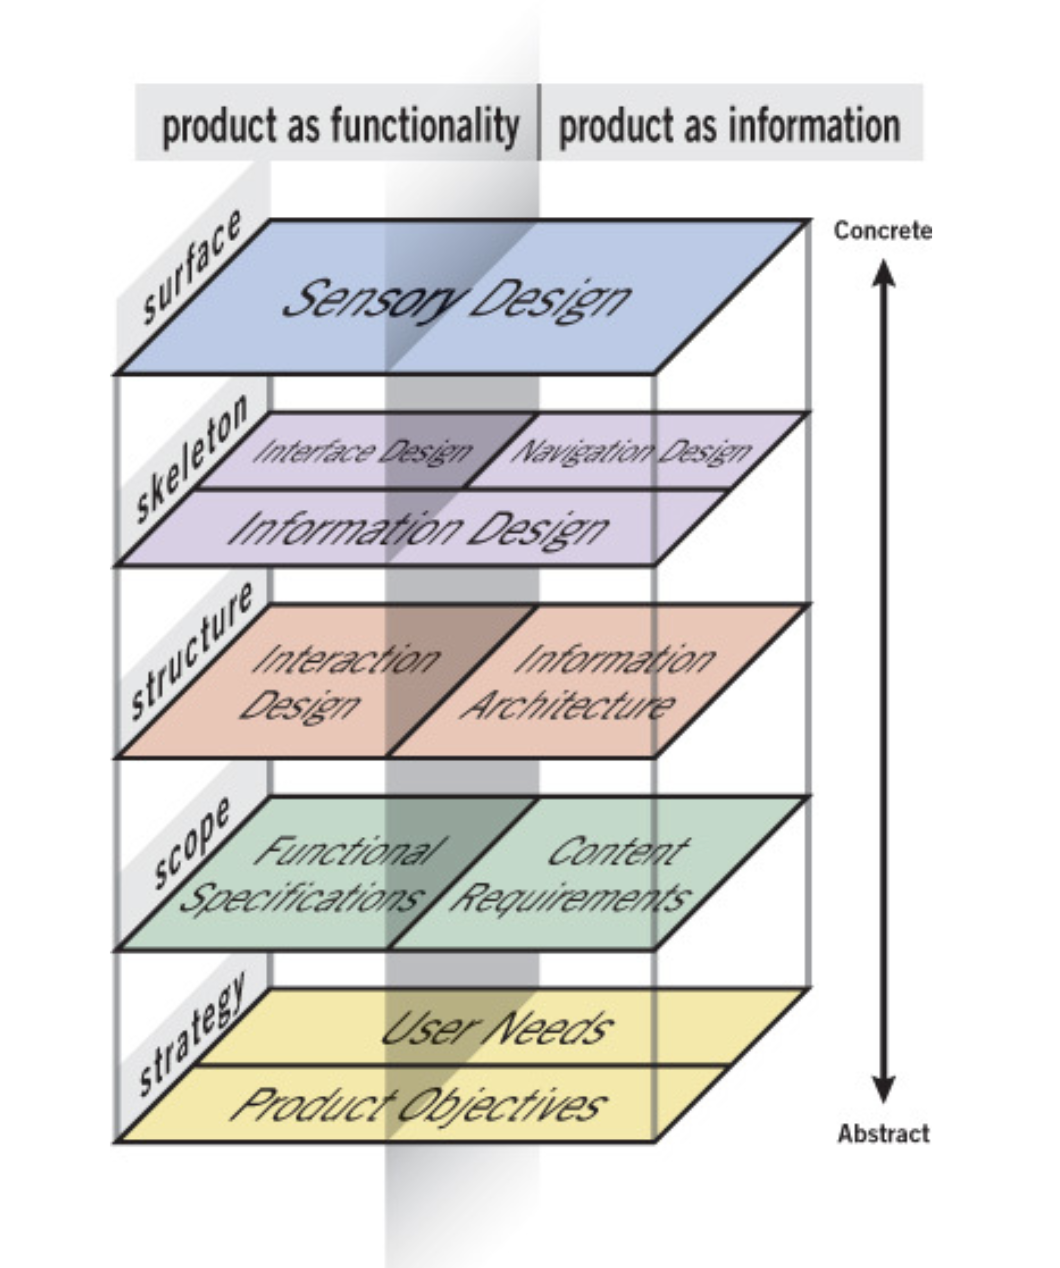
\includegraphics[width=100mm]{img/uxmodel.png}
    \end{center}
    \caption{GarretのUX五段階モデル\cite{garrett2010elements}}
    \label{fig:garretuxmodel}
  \end{minipage}
\end{figure}

\subsection{大規模開発に置けるユーザインタフェースデザイン}
資金や人的リソースが十分な大規模開発においてもデザイナがアプリのデザインについて専門的な知識を有しているとは限らない.デザイナを職業としている人の中でもGarretが述べている本来のデザインを忘れ,表層のデザインに注力してる場合が多く本来のデザインが一般に普及しているとは言えない.

また,デザイナよりもアプリに向き合っている時間が長いエンジニアの方がアプリのデザインについて専門的知識を持ち開発をおこなっている場合も多数ある.エンジニアの場合GarretのUX五段階モデルもさることながら,UIが実際に動く仕組みを理解している分,内部構造という面での専門知識を有してる場合も多い.
実際に日本経済新聞電子版のメンバーによるデザインに関する登壇では14個中全ての登壇がエンジニア,又はエンジニア経験のある人の登壇となっている.\cite{nikkeislide}


\subsection{個人開発に置けるユーザインタフェースデザイン}
個人開発アプリは大規模開発するほど収益が見込まれないものの,ニッチな消費者のニーズにあうさまざまなアプリケーションがアプリストアにリリースされている.
しかしながら資金,時間,人的リソースが十分にない個人開発では開発者がデザインの重要性について理解した専門家がいないことにより使い勝手が悪いものや,表層のデザインにのみ注力したアプリケーションがあり,消費者のニーズに答えられずにいる.


以上のことから,(1)現在は大規模な開発でしか行われていない専門性の高いユーザインタフェースデザインのハードルを下げること,(2)表層のデザインにとらわれずに奥深くのデザインに注力することができる手法を開発することが求められる.

\section{目的}
(1),(2) を満たすための,自動化で要素,優先度,グルーピングを使ったものを開発した.そして,開発したシステムの有用性を示した.
%
\section{本論文の構成}

本論文の構成を示す.

第\ref{chap:introduction}章では本研究の背景について述べた.第\ref{chap:prevresearch}章では関連研究と諸概念を整理する.第\ref{chap:pulsewave}章では要素,優先度,グルーピングからUIを自動生成する手法を提案し,第\ref{chap:pulsewave}章ではその手法をもとにiOS向けネイティブアプリケーションのコードを生成するシステムを提案する.そして,それらの有効性を示す.最後に,第\ref{chap:conclusion}章の結論では本研究を総括し,考察と展望を述べる.付録として,本研究で行った実験で得られたデータを添付する.
